\chapter{Introduction}
The loss of muscle mass with aging and disuse atrophy has been studied extensively. 
Accompanying the loss of muscle mass (\textit{sarcopenia}) is a disproportionately greater loss of muscle strength (\textit{dynapenia}) as we age~\cite{RNIGoodpaster}. 
The role of muscular and neural determinants of muscle force have been investigated in several human and animal studies~\cite{RNIBallak}.
In addition to these determinants, the role of the extracellular matrix (Figure~\ref{fig: ECM}) is also being increasingly recognized~\cite{RNIRamaswamy, RNIZhang}. 
For example, aging significantly alters proteins that transmit force both inside the muscle fibers~\cite{RNIHughes} and in the extracellular matrix~(ECM)~\cite{RNIKragstrup}, changing their content, orientation and composition. 
%*********************************************************
\begin{figure}[!ht]
\centering
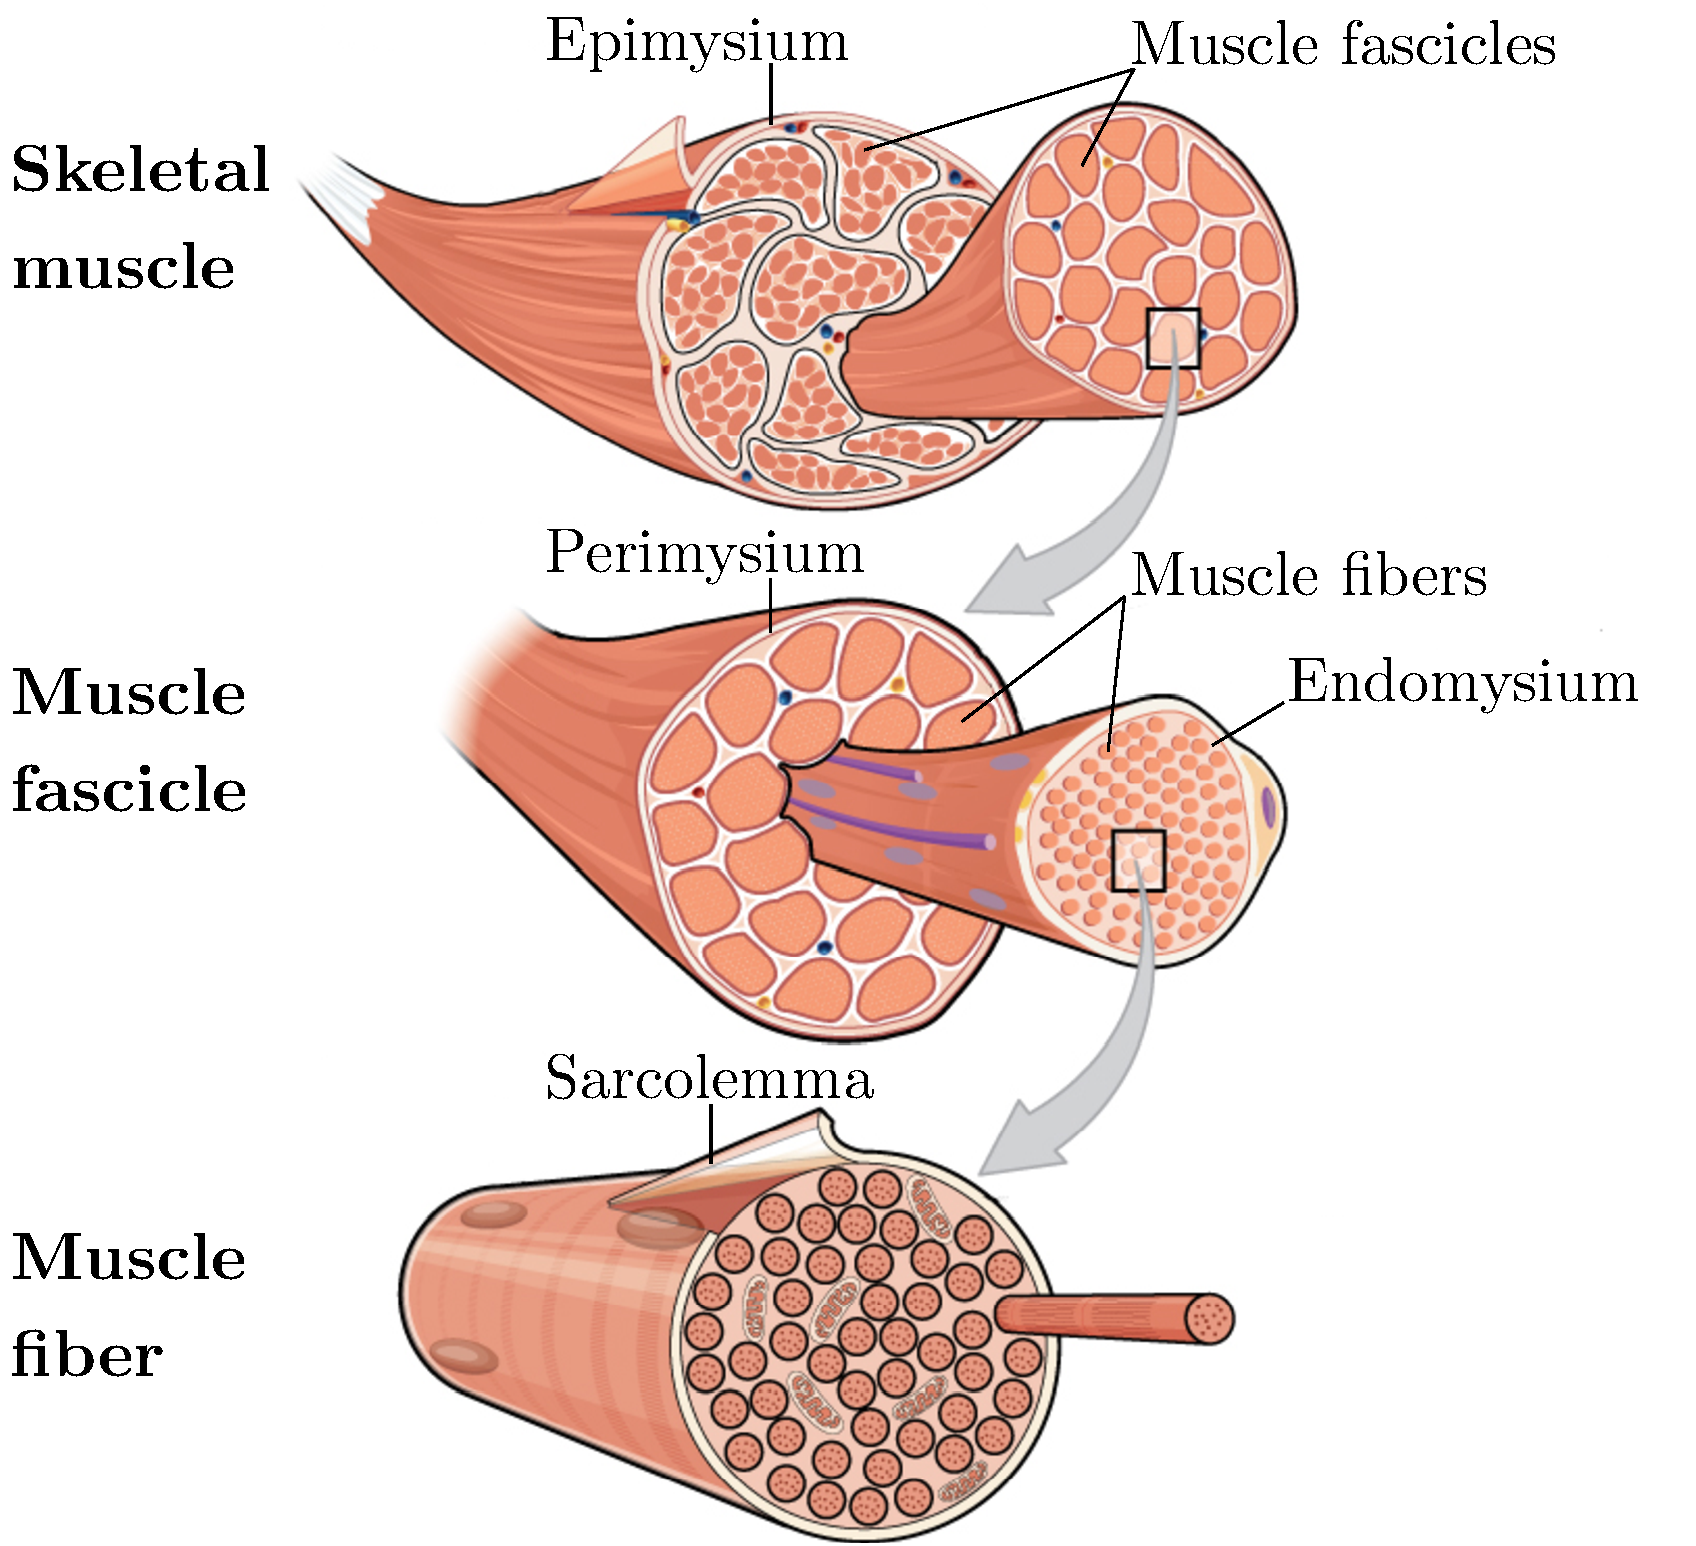
\includegraphics[scale=.4]{Figures/FIBER.pdf}
\caption[Skeletal muscle extracellular matrix]{Skeletal muscle extracellular matrix (ECM).}
\label{fig: ECM}
\end{figure}
%*********************************************************
The remodeling of the ECM may contribute to muscle weakness by impairing a muscle'��s capacity to transmit force. 
In young rodent muscles, at least 80\% of force transmission occurs laterally through the ECM~\cite{RNIHuijing}, whereas in frail old muscle, lateral transmission of force (LTF) through the ECM is reduced ~60\%~\cite{RNIRamaswamy, RNIZhang}. 
However, the contribution of the ECM to \textit{dynapenia} has never been comprehensively investigated in humans due to lack of non-invasive tools.
%-new paragraph-%

%-new paragraph-%
The non-invasive, \textit{in-vivo} nature of Magnetic Resonance Imaging (MRI) renders it particularly amenable to longitudinal studies of aging and disuse for both research and clinical purposes. 
MRI provides a unique non-invasive approach to monitor the \textit{in-vivo} changes in tissue deformation (strain or strain rate tensor) and its microarchitecture (diffusion modeleing).
%-new paragraph-%

%-new paragraph-%
My work explores age and atrophy related changes in strain rate parameters and their relationship to muscle force and to muscle structure.
Functional changes are studied by extraction of strain rate parameters from velocity encoded phase contrast images (VEPC).
Shear strain in the ECM has been postulated and validated with computational models to be the mechanism of lateral transmission of force. Thus mapping shear strain can potentially reflect changes in force transmission pathways.
It should be noted that shear strain will be influenced by the structural remodeling of the extracellular matrix.
Structural changes are studied using diffusion tensor imaging and the results are interpreted using bicompartmental and random permeable barrier diffusion models.